\begin{savequote}[8cm]
Everything comes to him who knows how to wait.

  \qauthor{--- Wolfgang Pauli }
\end{savequote}

\chapter{\label{ch:hnl}Heavy Neutral Lepton Sensitivity Estimation at the SFGD} 

\minitoc

    \section{Introduction}
        As a detailed review of heavy neutral lepton (HNL) would exceed the scope of this report, only a highly simplified introduction to HNL is given here. 
        The origin of the neutrino mass is still a mystery. 
        One intuitive solution is to extend the neutrino family to include heavy members, which are SM singlets and mix with the existing SM neutrinos via an extended PMNS matrix, thereby giving them the small masses observed via the see-saw mechanism~\cite{Abada:2007ux}. 
        In a simplified model, the HNL, $N$, is augmented to the SM neutrino family. 
        The neutrino flavour eigenstates, $\nu_\alpha$, can then be expressed as a linear combination of the SM neutrino mass eigenstates and the HNL:
        \begin{equation}
            \nu_\alpha = \sum_{i=1}^3 U_{\alpha i} \nu_i + U_{\alpha N} N,
        \end{equation}
        where $\alpha=e,\,\mu,\,\tau$, $\nu_i$ are the SM neutrino mass eigenstates, the $U_{\alpha i}$ are the elements of the PMNS matrix\footnote{They should have values close to the SM PMNS matrix elements, which has unitarity imposed.}, and $U_{\alpha N}$ is the new matrix entry describing the mixing of the HNL with the SM neutrinos to form the flavour eigenstates. 
        Due to this mixing with the SM neutrinos, when an SM neutrino is produced, e.g. $\nu_\mu$, it has a probability of $|U_{\alpha N}|^2$ to propagate as $N$.
        Hence, the intense neutrino beam in the long-baseline neutrino experiments can produce an intense flux of HNL, so the near detector of these experiments is a good place to look for HNL. 
        As $N$ is an SM singlet, it does not interact with the target materials in the detectors. 
        Its presence can only be inferred from its decay into SM particles, for example, $N\rightarrow l + \pi$, where $l$ is a lepton, such as an electron or a muon.
        The probability of the HNL decaying into a lepton, $\alpha$, is also proportional to the mixing element, $|U_{\alpha N}|^2$.
        These decay products can be detected by the sophisticated near detectors.
        Moreover, as the HNL signals come only from the HNL decay instead of interactions with the target materials, the detectable signal rate is proportional to the detector volume, while the SM neutrino background rate is proportional to the target mass.
        Hence, the ideal detector for HNL searches will have good detection capabilities with a large volume and a low density. 
        This is why T2K has searched for HNL~\cite{T2K:2019jwa} using the gaseous TPCs, a combined volume of about $7~\textrm{m}^3$, but not the scintillation detector, FGD, which has a considerably higher density and thus a significant background rate.
        As the ND280 upgrade replaces the P0D with SFGD and HAT, a combined volume of $8~\textrm{m}^3$, which are much better trackers than the P0D, they could be used in an HNL search as well.
        Since the HATs are gaseous TPCs as well, they are expected to have at least comparable performance to the TPCs. 
        Although the SFGD is a scintillation detector, it has improved reconstruction capabilities. 
        If it is capable of sufficiently suppressing the background rate, it can also be used in an HNL search, thereby improving the overall sensitivity of the T2K HNL search.
        Hence, the goal of this chapter is to demonstrate the feasibility of performing an HNL search using the SFGD.

        To perform an HNL search, a complicated chain of simulations is required, including the generation of an HNL flux based on the SM neutrino flux, the propagation of HNL and the decay of HNL. 
        The previous T2K search was based on a dedicated tool-set, \code{nd280HNLSim}, which was built only to search for $N\rightarrow l + \pi$ decay channels, where $l$ is a lepton. 
        It would require a large amount of efforts to extend it to include other production and decay channels. 
        Hence, I adapt the recently published general HNL package, \code{BeamHNL}~\cite{Plows:2022gxc}, to the T2K ND280 simulation to evaluate the sensitivity improvement brought by the upgrade.

        As the global reconstruction and systematics for the upgraded ND280 is not yet available, the result presented in this section is to demonstrate the successful implementation of the complete sensitivity estimation workflow, including the HNL simulation and selection, the background estimation, and the sensitivity extraction. 
        For this purpose, the $N\rightarrow\mu+\pi$ channel is chosen due to its similar event topology to the $\numuccopiop$ selection presented in Sec.~\ref{sec:sel-tl}.
        Moreover, the MC statistics used are relatively low for a quick demonstration of the implementation rather than a comprehensive sensitivity study, which does require higher statistics but would only be possible when the ND280 upgrade software is sophisticated enough to include as many decay channels as possible and to allow a comprehensive background estimation.

    \section{Implementation}
    \label{sec:hnl-impl}
        The simulation of HNL production and decay using \code{BeamHNL} is performed in several steps.
        Since \code{BeamHNL} is designed to be a cross-experiment package, it requires a standardized flux input in the \code{dk2nu} format. 
        The \code{dk2nu} file is a simple flat-tree ROOT file that must contain the minimally sufficient information for \code{BeamHNL} to function correctly.
        As the T2K flux is available in its own specific format, a conversion is necessary. 
        The required \code{dk2nu} variables and the corresponding conversion from variables in a T2K flux file are provided in Appendix~\ref{sec:app-hnl-dk2nu}.

        Using this input, the desired HNL production channels can be implemented by specifying a few additional parameters in a configuration \code{xml} file, \code{CommonHNL.xml}, located within the \code{GENIE} configuration directory. 
        These parameters are experiment-specific and must be set by the user. Details on how each parameter is set specifically for the T2K ND upgrade are provided in Appendix~\ref{sec:app-hnl-input}. 

        Before proceeding to subsequent steps, we validate the setup by feeding the T2K \code{dk2nu} file to \code{BeamHNL} and setting the HNL mass, $\mn$, to a small value, such as $1~\kev$. 
        The output HNL flux should closely mimic the SM flux. 
        The result is shown in Fig.~\ref{fig:hnl-fluxes}, where the orange dashed line ($\mn=1~\kev$) closely overlaps with the black solid line, which is directly plotted from the T2K input flux.  
        \begin{figure}[!htb] 
            \centering 		
            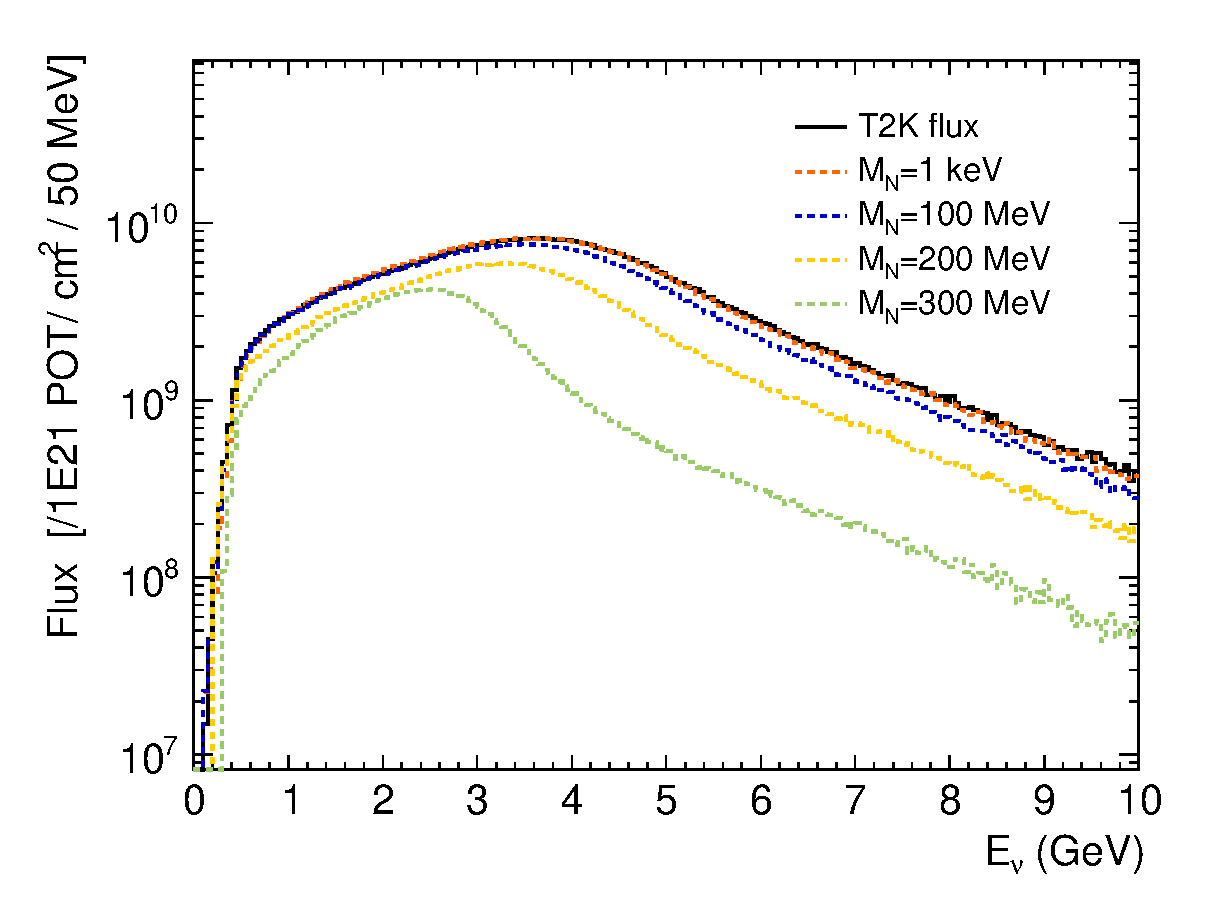
\includegraphics[width=\sgfigwid\textwidth]{figures/hnl/hnl_fluxes_less.eps}
            \caption{\label{fig:hnl-fluxes} HNL fluxes produced by \code{BeamHNL} for different $M_N$. The solid line is directly plotted from T2K input flux files. The dashed lines are \code{BeamHNL} outputs for different $\mn$. The $\mn=1~\kev$ curve agrees well with the T2K flux, validating the \beamHNL output. The curves for larger $\mn$ displaying apparent shape differences.} 
        \end{figure}
        After validation, the HNL mass is set to target values, e.g., $300~\mev$, to generate HNL events, which are then passed through the T2K simulation chain for selection development. 
        \begin{figure}[!htb] 
            \centering 		
            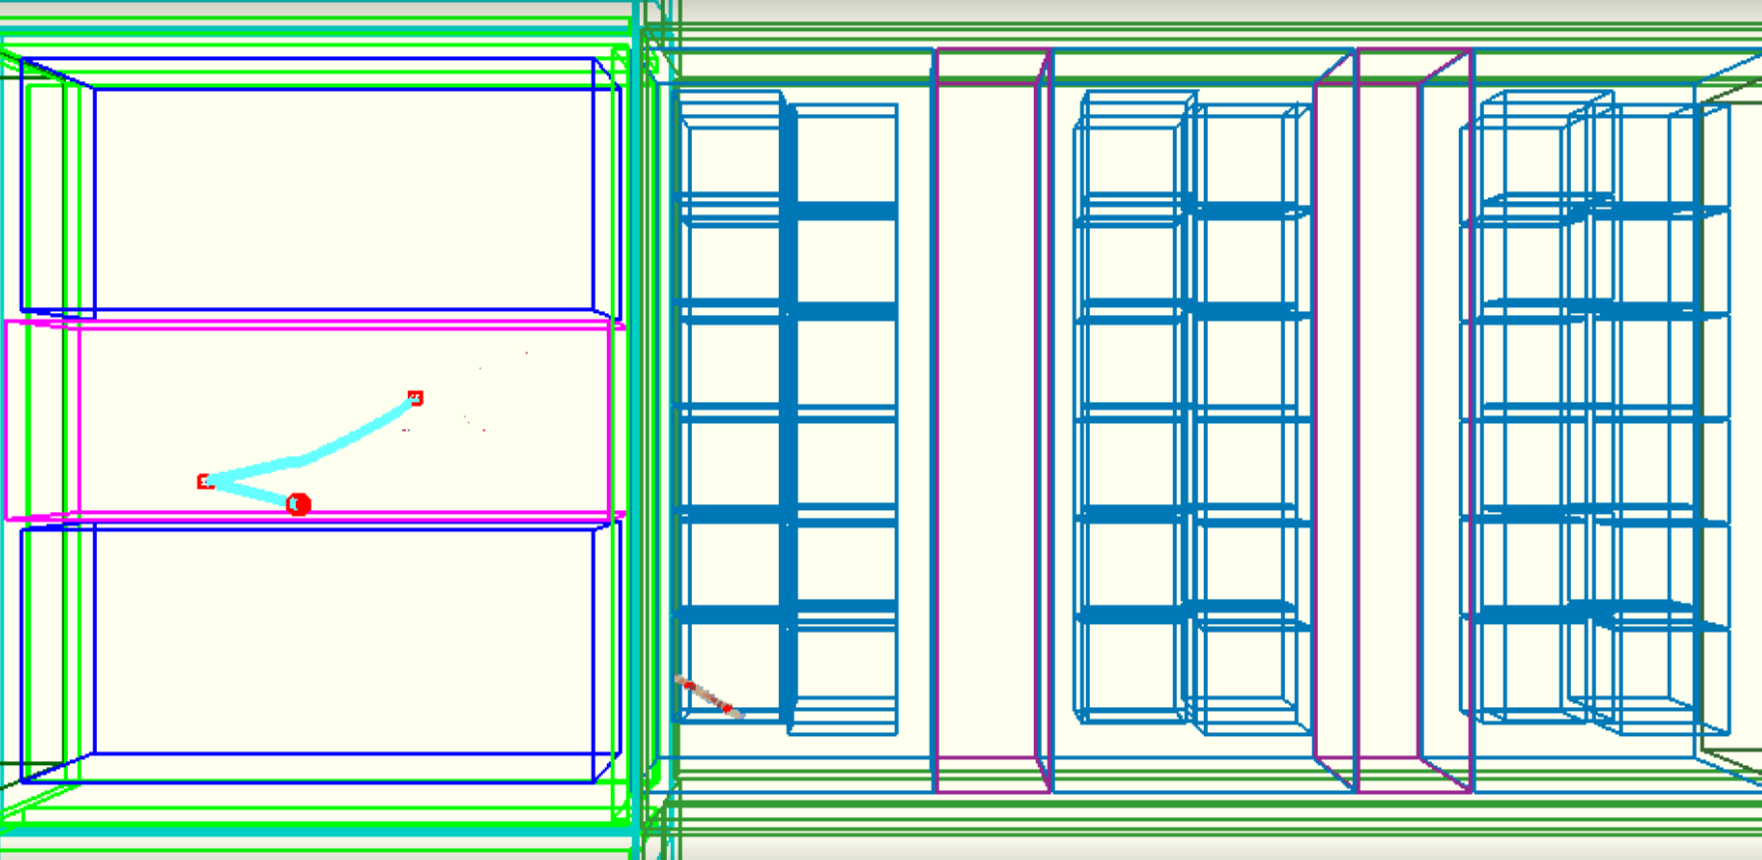
\includegraphics[width=\sgfigwid\textwidth]{figures/HNLEveDIs.png}
            \caption{\label{fig:hnl-evedis} A $N\rightarrow\mu+\pi$ event display in the upgraded ND280.} 
        \end{figure}

        With the successful interfacing between \code{BeamHNL} and the ND280 simulation, I proceeded to develop the selection for the $N\rightarrow\mu+\pi$ channel. 
        The steps are as follows:
        \begin{enumerate}
            \item \textbf{Basic T2K Event Quality Checks} 
            \item \textbf{Find SFGD Primary Vertex} 
            \item \textbf{Primary Track Count Cut} 
            \item \textbf{Escaping Muon Cut} 
            \item \textbf{Single Trackless Pion Cut}
            \item \textbf{Kink Cut}
            \item \textbf{$\mu$-$\pi$ Angle and Invariant Mass Cut}
            \item \textbf{$\mu$-$\pi$ $\dpt$ Cut}
        \end{enumerate}

        \textbf{Basic T2K Event Quality Checks} - A quality check ensures the event contains at least one reconstructed track.

        \textbf{Find SFGD Primary Vertex} - Identify a primary vertex in the SFGD. 
        Since the primary vertex for an HNL event does not necessarily include a muon, as in the $\numucc$ selection, the primary vertex should be identified independently from the primary muon. 
        All vertices are iterated through to record the number of tracks connected to each vertex, $n_{ptrk}$, and the length of the longest track connected to each vertex, $L_{max}$. 
        The vertex with the longest $L_{max}$ is selected as the primary vertex. 
        If more than one such vertex exists, the vertex with the largest $n_{trk}$ is selected. 
        If there is still more than one vertex, the vertex with the earliest time is selected.

        \textbf{Primary Track Count Cut} - For the target channel $N\rightarrow\mu+\pi$, there should be at most two primary tracks. Therefore, events with $n_{ptrk}>2$ are rejected.

        \textbf{Escaping Muon Cut} - This step identifies muons that escape the SFGD.

        \textbf{Single Trackless Pion Cut} and \textbf{Kink Cut} - These cuts are identical to those in the $\numuccopi$-Trackless selection, selecting a primary pion that has not undergone secondary interactions to ensure accurate reconstruction of its kinematics.

        \textbf{$\mu$-$\pi$ Angle and Invariant Mass Cut} - These are kinematic cuts that exploit the fact that SM events with one muon and one pion are mostly resonance events that have one more proton than HNL decays. Due to the additional proton, the opening angle between the $\mu$ track and the $\pi$ track, $\tmupi$, can vary widely, whereas in HNL decays, the angle is more collimated. Similarly, the invariant mass of the $\mu$-$\pi$ system, $\mmupi=(\pmu+\ppi)^2$, has a larger range compared to the HNL, which centres around the input value of $300~\mev$, as shown in Fig.~\ref{fig:hnl-mmupi}.
        The stark contrast is apparent in Fig.~\ref{fig:mmupi-mupiang}. To preserve the largest number of HNL events, the specific cuts applied are: $30^\circ < \tmupi < 90^\circ$ and $270~\mev<\mmupi<320~\mev$. 
        For a full sensitivity study over a wide range of HNL masses, the cut on $\mmupi$ needs to be relaxed, and the associated impacct will be investigated in the future.
        Note that the number of HNL events reaching this cut as shown in Fig.~\ref{fig:hnl-mmupi} is relatively small, as this selection effectively includes only muons escaping from the SFGD and travelling into the vertical TPC. 
        The statistics will increase when other sub-samples including muons in the other subdetectors are included when the global reconstruction is available.
        \begin{figure}[!htb]
           \centering
           \begin{subfigure}{\dbfigwid\textwidth}
                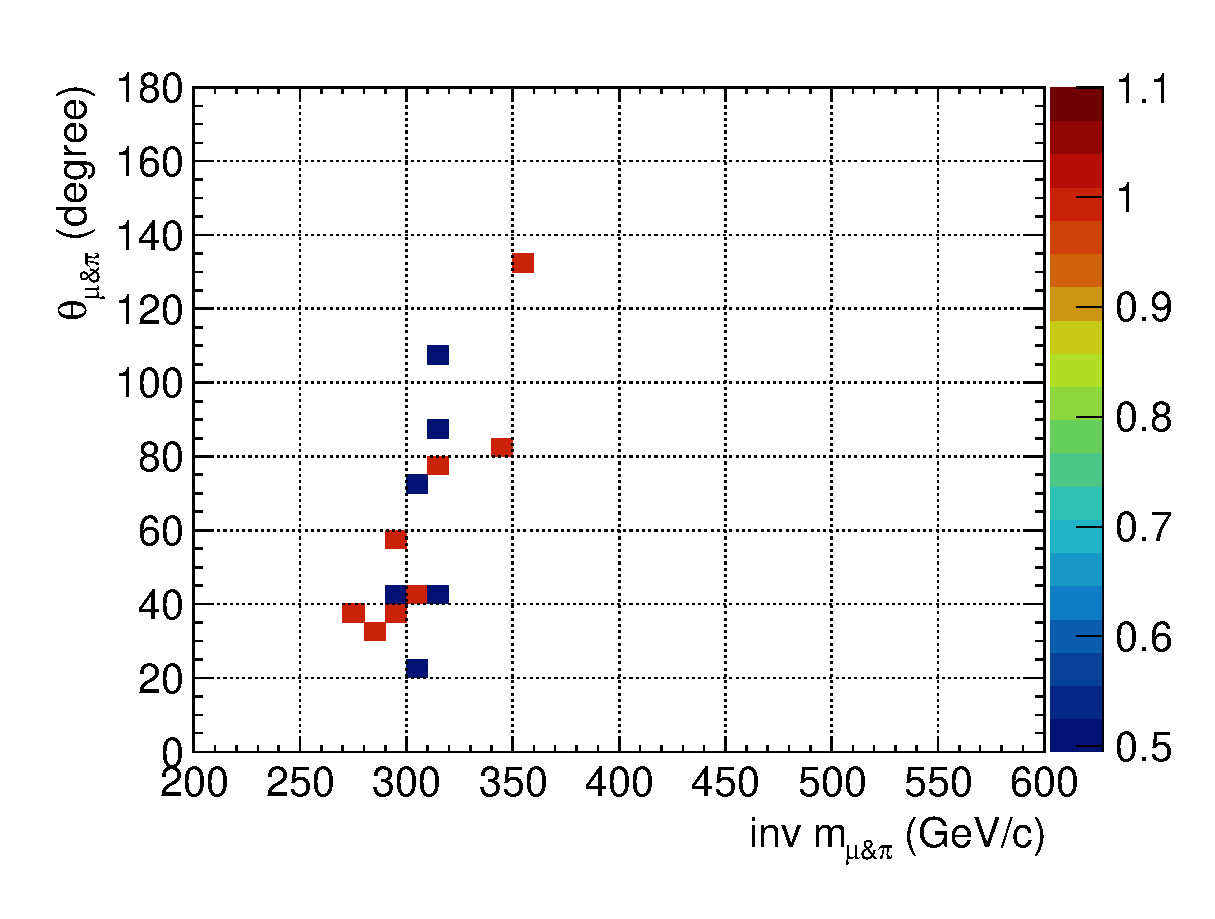
\includegraphics[width=\textwidth]{figures/hnl/hnl_sfgmu_mpinvm_colnor_vs_mpang_hist2d_al9_300.eps}
                \caption{HNL.}
                \label{fig:hnl-mmupi}
           \end{subfigure}
           \begin{subfigure}{\dbfigwid\textwidth}
                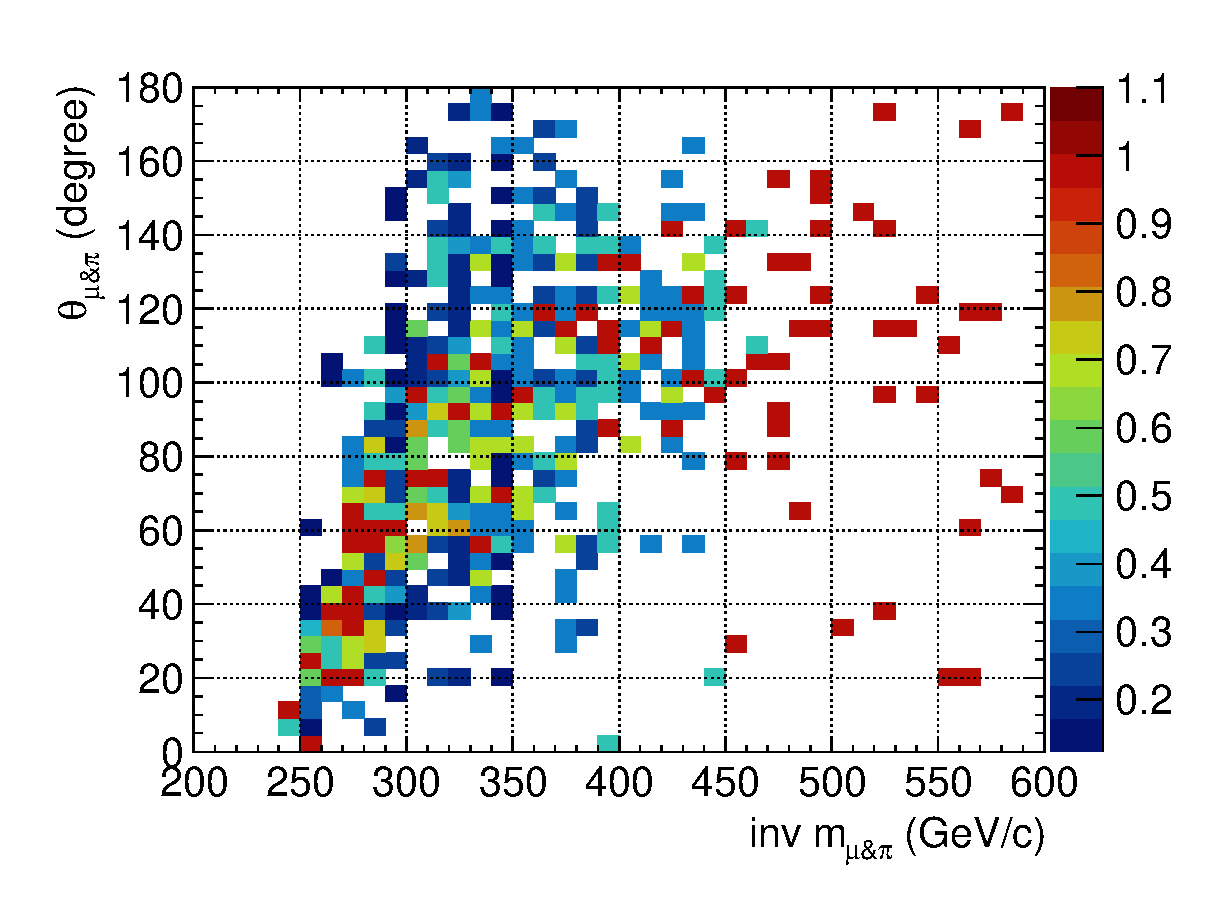
\includegraphics[width=\textwidth]{figures/hnl/hnl_sfgmu_mpinvm_colnor_vs_mpang_hist2d_al9_SM.eps}
                \caption{SM $\nu$.}
                \label{fig:sm-mmupi}
           \end{subfigure}
           \caption{$\tmupi$ plotted against $\mmupi$. The HNL events are concentrated near the rest mass of the HNL, while the SM events are more widely distributed.}
           \label{fig:mmupi-mupiang}
        \end{figure}

        \textbf{$\mu$-$\pi$ $\dpt$ Cut} - Similar to previous kinematic cuts, the net transverse momentum of $\mu$ and $\pi$ should be small, while for SM events it has a much larger range.
        To determine the appropriate cut value, the histograms of the net transverse momentum, $\dptmupi$, are plotted for both HNL and SM events, as shown in Fig.~\ref{fig:mmupi-dpt}.
        As the goal is to select HNL events while rejecting SM backgrounds, the histograms are only plotted for small $\dptmupi$ values, i.e., $\dptmupi<50~\mevc$. 
        The majority of SM events, with large $\dptmupi$, is thus not plotted in Fig.~\ref{fig:sm-mmupi}.
        In this particular case, applying the cut $\dptmupi<15~\mevc$ will retain eight HNL events and reject all SM backgrounds.
        A more realistic background estimation is given in the next subsection.

        \begin{figure}[!htb]
           \centering
           \begin{subfigure}{0.45\textwidth}
                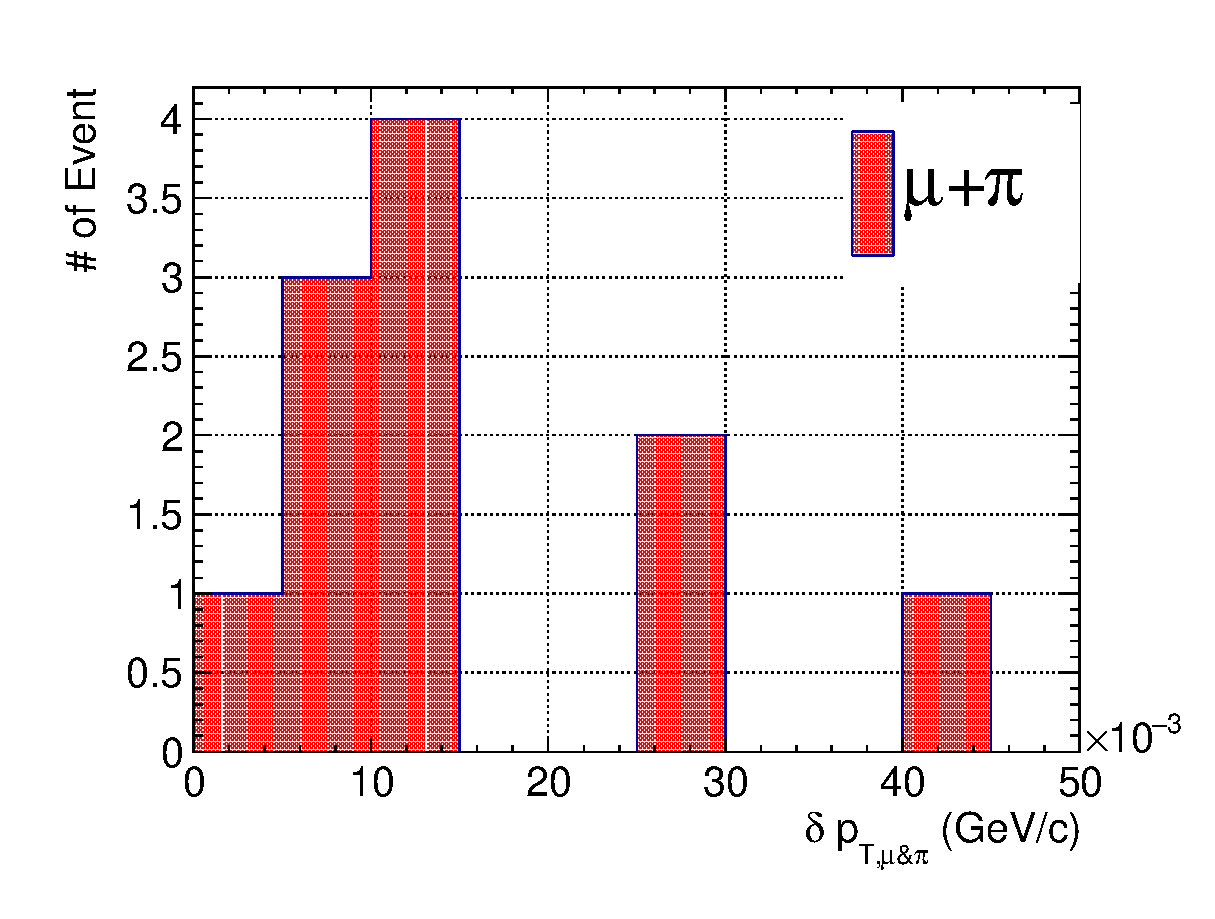
\includegraphics[width=\textwidth]{figures/hnl/hnl_sfgmu_mpdpt_stack_al9_300_aftmupikin.eps}
                \caption{HNL.}
                \label{fig:hnl-mupidpt}
           \end{subfigure}
           \begin{subfigure}{0.45\textwidth}
                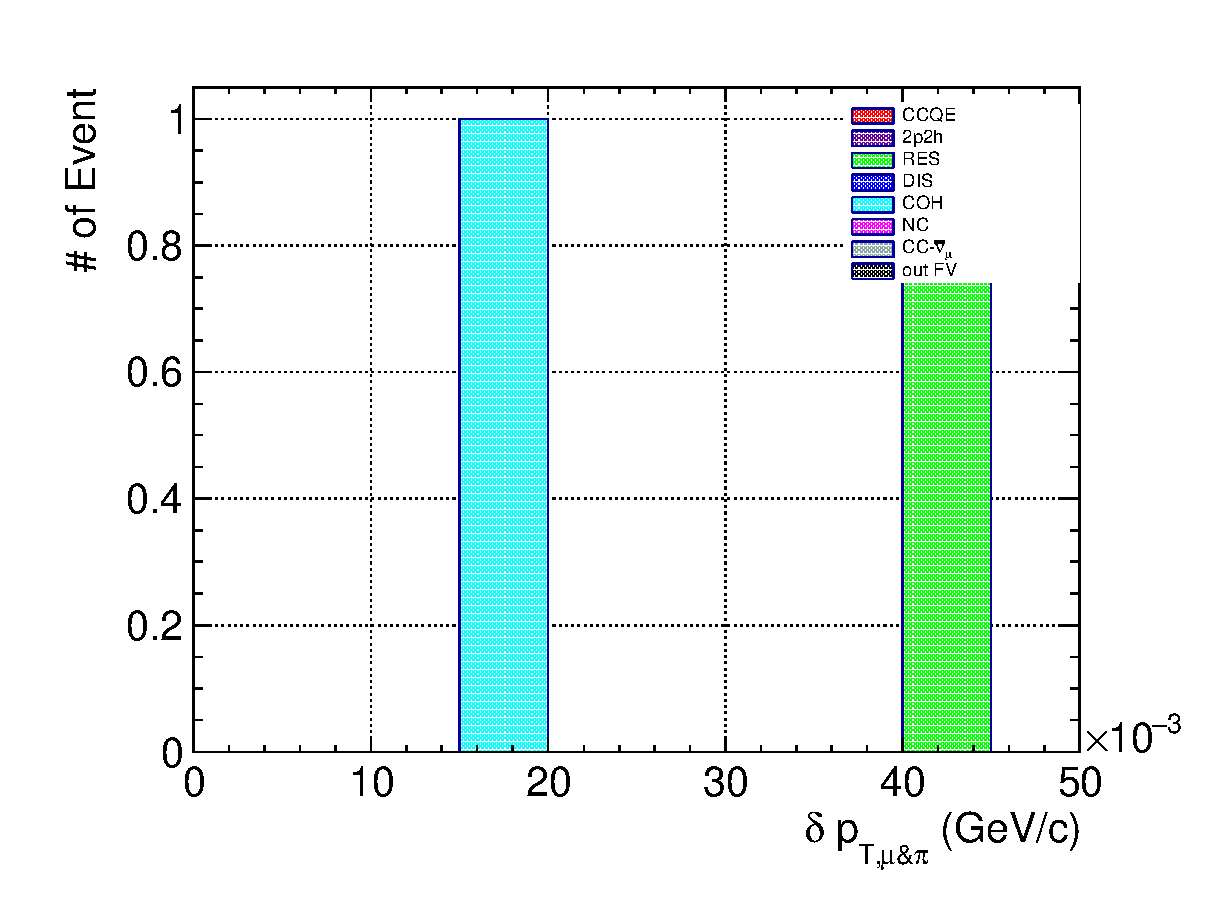
\includegraphics[width=\textwidth]{figures/hnl/hnl_sfgmu_mpdpt_stack_al9_SM_aftmupikin.eps}
                \caption{SM $\nu$.}
                \label{fig:sm-mupidpt}
           \end{subfigure}
           \caption{$\dptmupi$ distributions for HNL and SM $\nu$. HNL has significantly more events at small $\dptmupi$ values compared to SM $\nu$. The cut at $15~\mevc$ retains eight HNL events and rejects the remaining SM backgrounds. However,  this does not imply that this selection is background-free. A more realistic background estimation is given in the Sec.~\ref{sec:hnl-bkg}.}
           \label{fig:mmupi-dpt}
        \end{figure}

    
    \section{Background estimation}
    \label{sec:hnl-bkg}
        The previous T2K HNL search found that the coherent pion production is the dominant source for the $\mu\pi$ channel~\cite{T2K:2019jwa}.
        Hence, this background source is chosen in this subsection to demonstrate the background estimation procedure, while a comprehensive background estimation will be performed in the future when the upgrade software is ready.
        
        The $\dptmupi$ cut shown in Fig.~\ref{fig:sm-mupidpt} removes all coherent background. 
        However, the zero event is partly due to the small statistics used in this preliminary study.
        To properly estimate the coherent background, the full distribution of $\dptmupi$ before the last cut is fitted with a Cauchy distribution as shown in Fig.~\ref{fig:coh-bkg}.
        The number of expected background events is obtained by integrating the fitted curve from $0$ to the cut value, i.e. $15~\mevc$, which is evaluated to be $0.33$. 
        Although the fit quality is not perfect due to the low statistics, the procedure is still valid and can be applied to the full statistics when available.
        This background estimation procedure has not taken into account the systematic uncertainties, which needs to be evaluated by running toy simulations when the nd280 upgrade software is ready.
        \begin{figure}[!htb] 
            \centering
            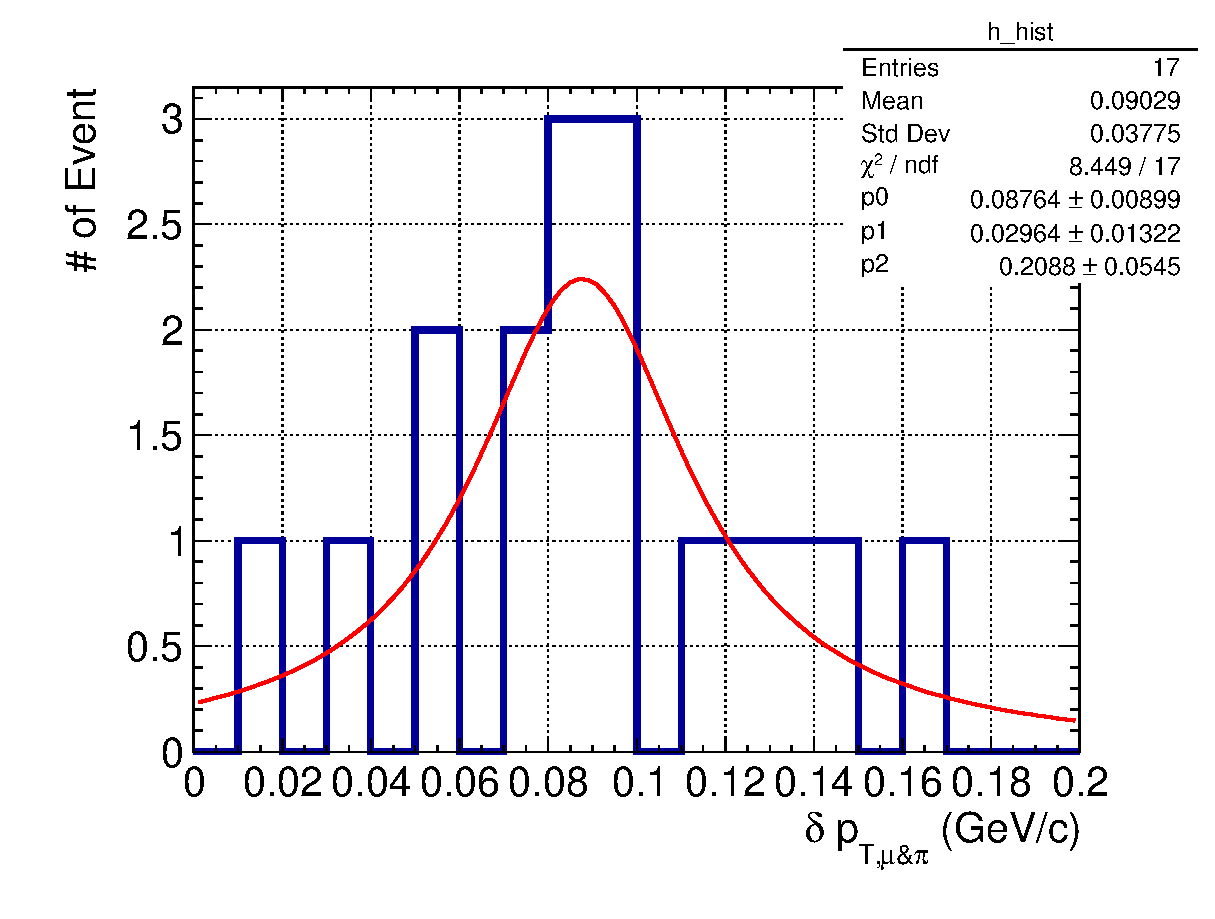
\includegraphics[width=0.5\linewidth]{figures/hnl/hnl_sfgmu_mpdpt_hist_al-1_SM_COH_zoom_fit.eps}
            \caption{$\mupidpt$ distribution fit for coherent pions surviving until the $\mupidpt$ cut. The background is estimated by integrating the fitted curve from $0$ to the cut value, $15~\mevc$, which is evaluated to be $0.33$.}
            \label{fig:coh-bkg}
        \end{figure}    
    
    \section{Sensitivity extraction}
        Sensitivity is extracted using the $CL_s$ method~\cite{Read:2002hq}.
        $CL_x$ is defined as $\textrm{Prob}(N\leq N_{\textrm{obs}}| \mu = x)$, i.e., the probability of predicting a number of events smaller than or equal to the number of observed events assuming model $x$. When $x=b$ or $x=s+b$, it corresponds to the background-only model or the signal plus background model, respectively.
        Then, $CL_s$ is defined as 
        \begin{equation}
            CL_s = \frac{CL_{s+b}}{CL_{b}} = \frac{\textrm{Prob}(N\leq N_{\textrm{obs}}| \mu = s+b)}{\textrm{Prob}(N\leq N_{\textrm{obs}}| \mu = b)} = \alpha,
        \end{equation}
        where $1-\alpha$ is the confidence level.

        For a target confidence level, $f$, one starts from $s=0$ and iterates with increasing $s$ to find the largest $s_{up}$ such that $\alpha < 1-f$. 
        Then, $s_{up}$ is the upper limit for the number of signal events at confidence level $f$ such that the background-only model is not rejected. 
        As for the value of $b$, it is conventional to use the median number of background events to evaluate $s_{up}$.
        After the $s_{up}$ is obtained, the limit on the desired parameter is extracted from its relation to $s_{up}$.
        In HNL searches, the parameter of interest is the mixing element $U_{\alpha N}$, where $\alpha$ is the lepton flavour of the decay products, i.e., $\mu$ or $e$.
        The production and decay of HNL are both proportional to the square of the mixing element.
        As the T2K flux is dominated by muon neutrinos and the decay channel explored is $N\rightarrow\mu+\pi$, the number of expected signal events is proportional to $|U_{\mu N}|^4$.
        Since only the squared magnitude of the mixing element can be extracted from the number of events, it is conventional to define $\umas=|U_{\alpha N}|^2$ as the parameter of interest.

        Specifically, for demonstration, the background is taken to be $b=0.33$ as evaluated in the previous subsection, leading to $s_{up}=2.3$ following the above $CL_s$ method.
        The number of observed events is $N_{\textrm{obs}}=8$, which is the number of HNL events surviving all cuts in Sec.~\ref{sec:hnl-impl}.
        However, one caveat is that the number of protons on target (POT) used to produce the HNL events is calculated from the \code{BeamHNL} output, which is approximately $0.81\times10^{21}$, while the background is estimatd from a POT of $1.0\times10^{21}$.
        Hence, the number of expected selected signal events will be $8/0.81\approx9.9$ for $10^{21}$ POT.
        This number of HNL events is generated with a mixing element of $U_{\mu} = 10^{-7}$, so the corresponding limit, $U_{up}$, on the mixing element, $U_{\mu}$, for observing $s_{up}=2.3$ events is calculated as 
        % $100,000$ \genie events were simulated using \code{BeamHNL}. 
        % The total number of protons on target (POT) required to produce these HNL events is calculated from \code{BeamHNL} output to be approximately $0.81\times10^{21}$ assuming $\umas=10^{-7}$. 
        \begin{align}
            \left(\frac{U_{up}}{10^{-7}}\right)^2 & =  \frac{2.3}{9.9} \\
            U_{up} & = 10^{-7} \times \sqrt{\frac{2.3}{9.9}} = 4.8\times10^{-8}.
        \end{align}

    \section{Discussion}
        This chapter has demonstrated the framework for the HNL sensitivity estimation using the SFGD has been successfully implemented.
        The crude sensitivity extracted from SFGD alone is approximately one order less sensitive the limit placed by the previous search, $U_{up}\approx4\times10^{-9}$, for $\mn=300~\mev$.
        There are two potential reasons for the lower sensitivity.
        Firstly, the current result includes only HNL decaying in SFGD, which has only about $1/3$ of the volume compared to the vertical TPCs, leading to at least a factor of $\sqrt{3}\approx1.73$ less sensitivity.
        Secondly, the selection only includes the muons escaping into the vertical TPC, while a considerable number of muons can escape into the HAT, so the sensitivity will increase when the HAT is included in the global reconstruction for selection development.
        While the background estimation appears optimistic, it is the signal to background ratio that is crucial for the sensitivity.
        As the MC statistics used is relatively low, the estimated number of signal events after the selection is susceptible to large statistical fluctuations. 
        Hence, the overall impact of including the SFGD to the HNL search can only be reliably assessed 
        with a larger sample and a full-scale background estimation when the ND280 upgrade software is ready.
        
        The next step is to extend the selection to the entire upgraded ND280 when the HAT reconstruction becomes available and to investigate the overall improvement in HNL sensitivity brought by the upgrade.
        Fig.~\ref{fig:hnl-hatevedis} shows a $N\rightarrow\mu+\pi$ event display in the Top HAT, demonstrating that the simulation of production and decay in HAT is successful. 
        \begin{figure}[!ht] 
            \centering 		
            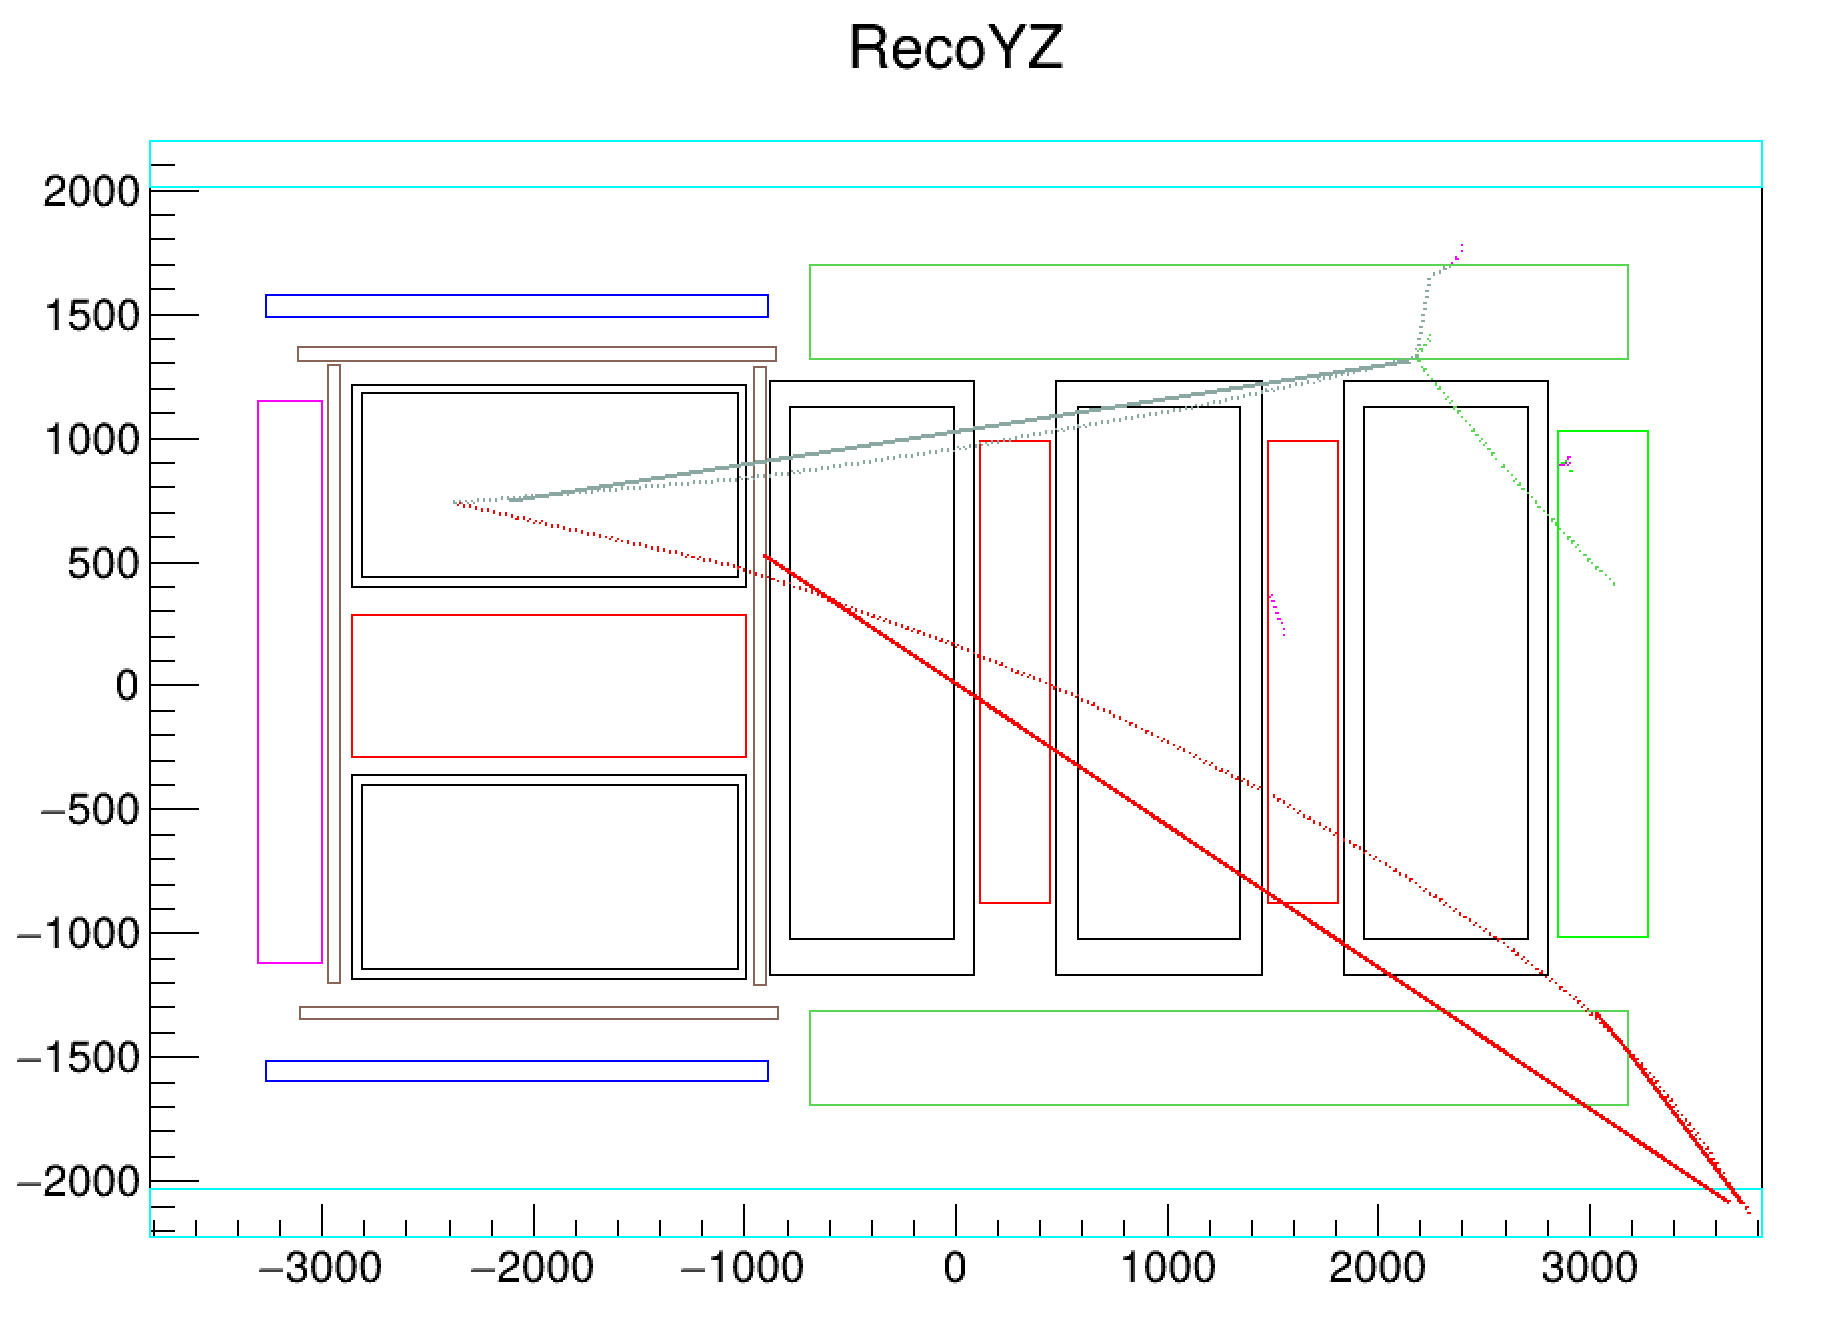
\includegraphics[width=0.7\textwidth]{figures/hnl/HATevedis.png}
            \caption{\label{fig:hnl-hatevedis} A $N\rightarrow\mu+\pi$ event display in the Top HAT.
            The solid lines are reconstructed tracks, and the dashed lines are true tracks.
            The red tracks correspond to a muon, and the grey tracks correspond to a pion.
            The pion is reconstructed satisfactorily, whereas the muon starting point is mis-reconstructed between the Top HAT and the first vertical TPC.
            }
        \end{figure}
        Unfortunately, the global reconstruction is not yet stable as shown by the mis-reconstruction of the muon in Fig.~\ref{fig:hnl-hatevedis}, so the sensitivity study of the full upgraded ND280 has to be reserved for future studies.
